% !TEX root=/home/tavant/these/manuscript/src/manuscript.tex

\chapter{Calculation of the SEE rate with and without saturation}
\label{an-SEE_exact}

The calculation of $\ratemaxw$ in \cref{eq-seemaxw} was done neglecting the saturation of $\proba$ at $\sigm$.
The exact value of  $\ratemaxw$ is proposed here including the saturation.
\cref{eq-seeyield} give, using the Maxwellian hypothesis

\begin{equation} \label{eq-SEE_sat}
  \ratemaxw(\Te) = \proba_0 + (1 - \proba_0) \frac{2 \Te}{\crover} + \frac{\int_{\ek_{\max}}^{+ \infty} (\probamax - \proba(\epsilon) f_M(\epsilon) d\epsilon}{1/4 n_e \bar{v}}
\end{equation}
with  $\ek_{\max}= \frac{\probamax - \proba_0}{1 - \proba_0} \crover $ is the minimum energy for which $\rate = \probamax$.
We obtain
\begin{align}  \label{eq-SEE_all}
  \ratemaxw(\Te) =& \proba_0 + (1 - \proba_0) \frac{2 \Te}{\crover} \\
  & + (\probamax - \proba_0) (\ek_{\max} + 1 )\exp(- \ek_{\max}) \\
  & + (\proba_0-1) (\ek_{\max}^2 +2\ek_{\max} + 2)\frac{\Te}{\crover} \exp(-\ek_{\max}) 
\end{align}

\Cref{fig-see_error} shows the evolution of the \ac{SEE} rate $\ratemaxw$ as a function of the electron temperature $\Te$ normalized by the crossover energy $\crover$.
On the left of \cref{fig-see_error}, we can see the comparison between the calculation neglecting the saturation  \cref{eq-seemaxw} and the calculation without neglecting it  \cref{eq-SEE_all}.
We can see that the two values are close up to $\frac{\Te}{\crover}\sim 1$, where the two values start to diverge from each other.
The right panel of \cref{fig-see_error} shows the evolution of the relative error as a function of $\frac{\Te}{\crover}$.
We can see that at $\frac{\Te}{\crover}\sim 1$, the error only equals 2\%.
\begin{figure}[hbtp]
  \centering
  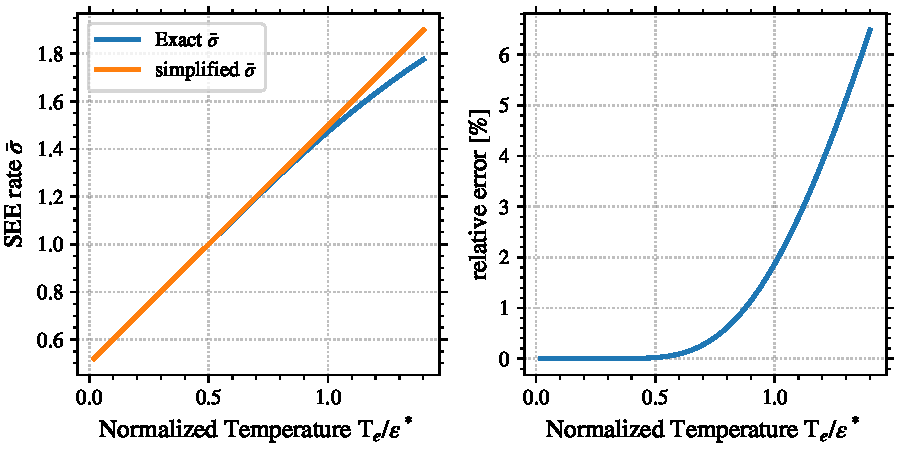
\includegraphics[width=0.9\textwidth]{SEE_rate_error_saturation.pdf}
  \caption{Evolution of the \acs{SEE} rate from a Maxwellian distribution function without and with the saturation at $\sigm$.}
  \label{fig-see_error}
\end{figure}

On the other hand, the \ac{SEE} rate $\rate$ crosses the threshold value of $\ratecr \simeq 1$ at $\Te/\crover = 0.5$.
We know that the a theoretical \ac{SEE} rate above $\ratecr$, the a potential well is present so that electrons are reflected to the wall, and therefore the effective \ac{SEE} rate is close to $\ratecr$.
Hence, the error between  \cref{eq-SEE_all} and \cref{eq-seemaxw} can always be neglected.
